\documentclass[11pt,a4paper]{article}
\usepackage{fontspec}
\usepackage{xeCJK}
\setCJKmainfont{STSong}
\setCJKsansfont{STHeiti}
\usepackage{amsmath,amssymb,amsthm}
\usepackage{mathtools}
\usepackage{bm}
\usepackage{booktabs}
\usepackage{array}
\usepackage{enumitem}
\usepackage{geometry}
\usepackage{xcolor}
\usepackage{tcolorbox}
\usepackage{algorithm}
\usepackage{algpseudocode}
\usepackage{pifont}
\usepackage{graphicx}
\usepackage{subcaption}
\usepackage{tikz}
\usetikzlibrary{arrows.meta,positioning,calc,fit,decorations.pathreplacing}
\usepackage[pdfencoding=auto,psdextra]{hyperref}

\geometry{margin=2.5cm}

\newcommand{\loss}{\mathcal{L}}
\newcommand{\E}{\mathbb{E}}
\newcommand{\R}{\mathbb{R}}
\newcommand{\KL}{\mathrm{KL}}
\newcommand{\N}{\mathcal{N}}
\newcommand{\adv}{\mathcal{A}}
\newcommand{\reward}{R}
\newcommand{\softmax}{\mathrm{softmax}}
\newcommand{\sg}{\mathrm{sg}}
\newcommand{\MoF}{\mathrm{MoF}}
\newcommand{\dom}{\mathrm{dom}}
\newcommand{\OOD}{\mathrm{OOD}}
\newcommand{\const}{\mathrm{const}}
\newcommand{\OPD}{\mathrm{OPD}}
\newcommand{\PG}{\mathrm{PG}}
\newcommand{\Path}{\mathrm{path}}

\theoremstyle{definition}
\newtheorem{definition}{定义}
\newtheorem{remark}{注}
\newtheorem{proposition}{命题}
\newtheorem{corollary}{推论}
\newtheorem{lemma}{引理}
\newtheorem{theorem}{定理}
\newtheorem{example}{例}

\title{\textbf{Mixture of Flows}}
% \author{Bowen Ping}
\date{}

\begin{document}
\maketitle

\begin{abstract}
本文研究如下问题：将 $K$ 个针对不同 reward objective 微调的 specialist
扩散 teacher $\{v^{(k)}\}_{k=1}^K$ 蒸馏到\emph{单个} student 中，使该 student
在每个 reward 上达到\emph{对应 teacher 水平}的 in-domain 性能，同时在 OOD
（out-of-distribution）reward 上获得跨目标增益。我们给出三点观察：

\textbf{(i)}~标准 On-Policy Distillation (OPD) 应用于扩散模型时可分解为
\emph{path-wise} MSE 项与 \emph{policy-gradient} (PG) 项；当 teacher 作为
target 时，PG 项的期望贡献为零，因此\emph{单纯的 velocity MSE 即足够}。

\textbf{(ii)}~朴素多 teacher OPD 有两类自然失败模式：
\emph{route-by-source} 把 student 钉死在单 teacher 上限，无 OOD 增益；
\emph{averaging} 由 Jensen 不等式导致 in-domain 严格下降，OOD bonus 极小。

\textbf{(iii)}~我们\emph{有可能}构造一个更好的 target：取可学习的凸组合
$v_\lambda = \sum_k \lambda_{k,t,s,c}\,v^{(k)}$，权重以 (teacher, time,
source, prompt) 为条件。由于合法 flow-matching velocity field 的凸组合
仍是合法 velocity field，$v_\lambda$ 是合法Flow-Matching模型，可以在小型混合参数
空间上用 RL（DiffusionNFT 或 Flow-GRPO）调优。Student 通过纯 pathwise
MSE 从 $v_{\lambda^*}$ 蒸馏。

本框架给出一个\emph{构造性的} Level-1 in-domain 保证：student 在每个
in-domain dataset 上的期望 reward 至少不低于对应单 teacher。但我们也
证明 OOD 严格超越在一般情况下\emph{无法保证}。
实验设置（三个 teacher 已训练到 GenEval=0.958, OCR=0.953,
PickScore$\approx$24.13）以及初步实验观察到的失败模式清单。
\end{abstract}

\tableofcontents
\newpage

%% ============================================================
\section{引言}
\label{sec:intro}
%% ============================================================

\subsection{动机}

现代文生图扩散模型的微调已成为多目标问题：人类偏好（如 PickScore）、
组合准确性（如 GenEval）、文字渲染保真度（OCR）都是想要的能力，每个
都有自己的 reward model 和训练集。RL 微调（Flow-GRPO, DiffusionDPO,
DiffusionNFT）通常只优化\emph{单个} reward，所以实际流水线是分别训练 $K$
个\emph{专家} LoRA teacher $\{v^{(k)}\}_{k=1}^K$——单个 reward 上的
in-domain 表现强，但没有一个可部署的统一 artifact 在所有 reward 上都强。

接下来的自然问题：\emph{能否把这 $K$ 个 teacher 蒸馏成一个 student}，让该
student 既匹配每个 teacher 的 in-domain 强度，又能获得跨目标增益？我们
约定：在 prompt set $\mathcal{P}_s$ 上评估 reward $R_s$ 称为
\textbf{in-domain} 性能（$v^{(s)}$ 是为该 set 训练的 teacher），在
$\mathcal{P}_s$ 上评估 reward $R_j$（$j \neq s$）称为 \textbf{OOD} 性能。

\subsection{已有方案的失败模式}

两个由 OPD 派生的自然 baseline，以对称的方式失败：

\begin{itemize}[leftmargin=1.5em]
\item \textbf{Route-by-source}。每个 prompt 路由到 source-matched
teacher，student 只拟合该 teacher。Student 性能上界由对应单 teacher 决定；
\emph{无} OOD 增益，因为 cross-teacher 信息从未进入梯度。

\item \textbf{Averaging}。Student 拟合算术平均
$\bar v = \tfrac{1}{K}\sum_k v^{(k)}$。由 Jensen 不等式（结合
velocity-MSE 与 KL distillation 的等价关系），student 在每个
in-domain 配对 $(s, s)$ 上\emph{严格退化}于单 teacher baseline；OOD
往往略有提升但增益小且不必然成立。
\end{itemize}

两种模式共享同一根本约束：一旦 target 给定，student 的 velocity field
在每个 $(x, t)$ 点上被刚性锁定。\textbf{没有用于跨目标协同的余量}——例如
让某个 teacher 在早期 timestep 主导 $R_s$（layout），另一个在晚期主导
$R_j$（texture）。

\subsection{我们的方法}

\textbf{先构造一个更好的 teacher 再蒸馏}。具体地，
\begin{equation}
v_\lambda(x,t,c) \;=\; \sum_{k=1}^{K}\lambda_{k}(t,s(c),c)\,v^{(k)}(x,t,c),
\qquad
\sum_k \lambda_k = 1,\;\;\lambda_k\geq 0,
\label{eq:mof_intro}
\end{equation}
其中 $\lambda$ 同时依赖 teacher index $k$、timestep $t$、source label
$s(c)$ 和（可选的）prompt embedding $c$。我们仅优化这些 $\lambda$，在
\emph{velocity 输出空间}用 RL 在复合 reward 上调优，然后用纯 pathwise
MSE 把最终的 $v_{\lambda^*}$ 蒸馏成一个 student LoRA。

\subsection{贡献与文章结构}

\begin{enumerate}[leftmargin=1.5em]
\item \textbf{方法（\S\ref{sec:method}）}：三阶段流水线——OPD pathwise
sufficiency $\to$ MoF target construction by RL $\to$ on-policy
distillation——把"找到好的凸权重"与"把它编码进单个 LoRA"解耦。混合
搜索空间仅 $K\times T\times S \sim 10^2$ 个参数（LUT）或 $\sim 10^6$
（router），相比 $10^7$--$10^9$ 的 student 参数微不足道。

\item \textbf{理论（\S\ref{sec:theory}）}：
\emph{构造性}的 Level-1 in-domain 保证（\S\ref{ssec:level1}）；时间
互补性下\emph{条件性}的 Level-2 in-domain 严格超越（\S\ref{ssec:level2}）；
关于 OOD 严格超越的\emph{负面定理}（\S\ref{ssec:no_ood}），揭示 in-domain
与 OOD 间的不对称性，附带三类充分条件；NFT 的 $\beta$ 消去性质分析
（\S\ref{ssec:beta_cancel}）；以及蒸馏 gap 抹消的讨论
（\S\ref{ssec:distill_gap}）。

\item \textbf{实验（\S\ref{sec:experiments}）}：实验协议包含三个 Flow-DPPO
teacher（GenEval/OCR/PickScore 分别达到 0.958/0.953/24.128）、四种混合
模块变体（LUT, LUT-SA, Time Router, adaLN/MLP Router）、两种 RL 选择
（DiffusionNFT, Flow-GRPO），以及对 OOD bonus $\gamma$ 与初始化的消融。
我们报告了一个初步失败模式——\emph{PickScore-dominance} 效应，神经
router 因 PickScore 的 \texttt{applicable\_sources} 覆盖所有 source（其他
是 domain-specific）而非对称地放大其 PickScore 信号。
\end{enumerate}

%% ============================================================
\section{背景}
\label{sec:background}
%% ============================================================

\subsection{Flow matching 与符号}

设 $x_0 \sim p_{\text{data}}$, $x_1 \sim \N(0, I)$。Flow matching
参数化一个 velocity field $v_\theta(x, t, c)$ 使 ODE
$\dot x_t = v_\theta(x_t, t, c)$ 把噪声分布运输到数据分布。标准训练
loss：
\begin{equation}
\loss_{\text{FM}}(\theta) = \E_{x_0,x_1,t}\!\left[
\big\| v_\theta(x_t,t,c) - (x_1 - x_0) \big\|_2^2
\right],\qquad x_t = (1-t) x_0 + t\,x_1.
\label{eq:fm}
\end{equation}
Teacher 是冻结的 $v^{(k)}$（通常是 base flow model 上的 LoRA snapshot）。
我们用 $k \in \{1, \ldots, K\}$ 索引 teacher，$s \in \{1, \ldots, S\}$
索引 source（每个 source 有 in-domain reward $R_s$），$i \in \{0, \ldots,
T-1\}$ 索引 timestep，$\mathcal{P}_s$ 表示 per-source prompt set。
记号 $f_j^{(s)}(\lambda) \triangleq
\E_{p \sim \mathcal{P}_s}[R_j(\mathrm{ODE}(v_\lambda; x_T, p))]$
表示 mixing $\lambda$ 在 prompt set $\mathcal{P}_s$ 上获得的 reward $R_j$
期望。

\subsection{OPD：pathwise vs.\ policy-gradient}
\label{ssec:opd_decomp}

设目标是把 teacher $v^{\mathrm{tgt}}$ 蒸馏到 student $v_\theta$。设
$q_\theta$ 是 student 的轨迹分布，$q_{\mathrm{tgt}}$ 是 teacher 的。最小化
path-wise KL $\KL(q_\theta \| q_{\mathrm{tgt}})$ 有标准分解（参考 OPD
文献）：
\begin{equation}
\nabla_\theta \KL(q_\theta\|q_{\mathrm{tgt}})
\;=\;
\underbrace{\E_{q_\theta}\!\left[\sum_i\frac{1}{2\bar\sigma_i^2}\nabla_\theta\| \mu_\theta^i - \mu_{\mathrm{tgt}}^i \|^2\right]}_{\text{pathwise}}
\;+\;
\underbrace{\E_{q_\theta}\!\left[\sum_i \big(\log q_\theta - \log q_{\mathrm{tgt}}\big)\nabla_\theta\log q_\theta\right]}_{\text{policy-gradient (REINFORCE)}}.
\label{eq:kl_decomp}
\end{equation}

\begin{proposition}[PG 项期望贡献为零]
\label{prop:pg_zero}
在标准假设下（密度光滑，方差有限）且 $v_\theta$ 的参数化使每个中间
step 满足 $\E_{q_\theta}[\nabla_\theta \log q_\theta] = 0$（score-function
identity），则~\eqref{eq:kl_decomp} 中 policy-gradient 项在 pathwise
梯度已应用的条件下\emph{均值为零}，仅贡献方差。
\end{proposition}

\begin{proof}[证明草图]
定义 $r_i := \log q_\theta - \log q_{\mathrm{tgt}}$，
$g_i := \nabla_\theta \log q_\theta$。由 score-function identity
$\E[g_i] = 0$。若在 $q_\theta$ 下 $r_i, g_i$ 独立（或弱相关），则
$\E[r_i g_i] \approx \E[r_i] \E[g_i] = 0$。在扩散设定中，sampling
轨迹由 $v_\theta$ 生成，pathwise 项已经把 $\mu_\theta^i$ 校正到
$\mu_{\mathrm{tgt}}^i$ 方向，所以\emph{剩下的} REINFORCE 信号是高方差
噪声而非方向性偏置。经验上（OPD 文献已确立）：单纯使用 pathwise 项
训练与使用完整 KL 梯度训练收敛到同一不动点。
\end{proof}

\textbf{实践推论}：本流水线中的 distillation 退化为纯 velocity MSE
（无 log-prob、无 importance ratio、无 clipping）。这正是
\texttt{trainers/mof/distill.py} 的实现（参见
\texttt{mof\_two\_stage\_pipeline.tex}）。

\subsection{Flow-matching velocity 的凸组合仍是 flow-matching velocity}

\begin{proposition}[FM 的凸闭性]
\label{prop:convex_fm}
若 $v^{(1)}, \ldots, v^{(K)}$ 都是合法 flow-matching velocity field（各自
满足连续性方程 $\partial_t p_t + \nabla \cdot (p_t v^{(k)}) = 0$），则
对任意 $\lambda \in \Delta^{K-1}$：
\begin{equation}
v_\lambda \;=\; \sum_k \lambda_k v^{(k)}
\end{equation}
也是合法 flow-matching velocity field。
\end{proposition}

\begin{proof}
连续性方程关于 $v$ 是线性的；解的凸组合仍是解（形式上，对应的
marginal density 是 teacher marginal 的凸组合）。
\end{proof}

这是 MoF 的关键结构性事实：\emph{任意} per-timestep 混合 $v_\lambda$ 都
定义一个合法扩散模型，其 ODE 是 well-posed 的，轨迹可被采样、打分、
蒸馏。

\subsection{多 teacher OPD 的失败模式}
\label{ssec:opd_failures}

记 $f_j^{(s)}(\theta)$ 为蒸馏后 student 在 prompt set $\mathcal{P}_s$
上的 reward $R_j$ 期望。

\paragraph{Route-by-source.}
训练 $K$ 个独立 student，或一个根据 $s(p)$ 切换 teacher 的 student。
最优 student velocity 为 $v_\theta^*(x, t \,|\, p \in \mathcal{P}_s) =
v^{(s)}(x, t)$，故 $f_s^{(s)}(\theta^*) \approx f_s^{(s)}(v^{(s)})$
（in-domain 精确匹配 teacher，仅有蒸馏 gap），且
$f_j^{(s)}(\theta^*) \approx f_j^{(s)}(v^{(s)})$（OOD 直接继承 teacher
$s$ 的 OOD 分数——无 cross-teacher transfer）。\emph{无 OOD 增益}。

\paragraph{Averaging.}
训练 student 拟合 $\bar v = \tfrac{1}{K} \sum_k v^{(k)}$。最优 student
是 $v_\theta^* = \bar v$。对足够"尖锐"的 reward 应用 Jensen 不等式，
$f_s^{(s)}(\bar v) < f_s^{(s)}(v^{(s)})$ 对每个 in-domain 配对 $(s, s)$
成立（\emph{严格 in-domain 退化}）。OOD 通常略有提升（因为 $\bar v$
混合了 teacher 行为），但增益小且不一定成立。

\medskip

\begin{tcolorbox}[colback=red!5,colframe=red!50,title=两种失败模式
共享同一结构性原因]
Student 的最优 velocity 被 target 构造方式刚性锁定：route 选 teacher
凸包的一个顶点 ($v^{(s)}$)，averaging 选重心。两者都没用上
命题~\ref{prop:convex_fm} 给出的 per-timestep 余量。要利用它，权重必须
\emph{学出来}，依据是 reward landscape 上真正能帮上忙的方向——这正是
MoF 的核心想法。
\end{tcolorbox}

%% ============================================================
\section{方法：Mixture of Flows}
\label{sec:method}
%% ============================================================

\subsection{MoF 构造}
\label{ssec:mof_def}

\begin{equation}
v_\lambda(x,t,c) \;=\; \sum_{k=1}^{K}
\lambda_k\!\big(t,\,s(c),\,c;\,\psi\big)\,v^{(k)}(x,t,c),
\qquad
\lambda_k = \frac{\exp(\ell_k/\tau)}{\sum_{k'}\exp(\ell_{k'}/\tau)}.
\label{eq:mof_def}
\end{equation}
其中 $\psi$ 是\emph{可学习的混合参数}的小集合（logits $\ell$ 经 softmax
归一化）。Teacher 全部冻结且 detached。

我们用五种表达力递增的方式实例化 $\lambda$，每种由
\texttt{trainers/mof/common.py} 中的一个 \texttt{MoFMixingModule}
子类实现：

\begin{center}
\renewcommand{\arraystretch}{1.3}
\footnotesize
\begin{tabular}{@{}p{2.6cm}p{4.5cm}p{4.5cm}@{}}
\toprule
\textbf{模块} & \textbf{$\ell$ 的形式} & \textbf{说明} \\
\midrule
LUT & $\ell\in\R^{K\times T\times S}$ & Per-source \& per-step 查表；$K{\cdot}T{\cdot}S\sim 10^2$ 参数。 \\
LUT-SA & $\ell\in\R^{K\times T}$ & 源无关；按 $S$ 维广播。诊断 baseline。 \\
Time Router & $\ell = \mathrm{MLP}(t)$ & $t$ 上连续；无 prompt conditioning。 \\
adaLN Router & $\ell = \mathrm{MLP}(\mathrm{adaLN}(t,c))$ & adaLN 融合（DiT 风格）。 \\
MLP Router & $\ell = \mathrm{MLP}([\mathrm{TE}(t)\Vert c_{\text{pool}}])$ & 拼接后过 MLP。 \\
\bottomrule
\end{tabular}
\end{center}

我们统一用 $\psi$ 表示参数集（无论是 $K\!\times\!T\!\times\!S$ logits
还是 router 网络权重）。$\psi$ 的参数量比 student 参数小至少四个数量级。

\subsection{二阶段流水线}
\label{ssec:two_stage}

\paragraph{Stage 1（在 $\psi$ 上做 RL）。}
我们把 $v_\lambda$ 当作 policy，用 RL 在复合 reward 上优化 $\psi$。由
命题~\ref{prop:convex_fm}，$v_\lambda$ 是合法 FM，因此任何支持
flow-matching policy 的 RL 算法都适用。我们用 \textbf{DiffusionNFT}
作为主算法（基于 advantage 重权的 path-wise 重建 loss；细节见
\S\ref{ssec:nft_choice} 和 \texttt{mof\_two\_stage\_pipeline.tex}）。
备选：\textbf{Flow-GRPO}（PPO 风格 ratio + 随机 CPS scheduler）作为
消融对照。

\paragraph{Stage 2（把 $v_{\lambda^*}$ 蒸馏到 student LoRA）。}
Stage 1 完成后，$\psi^*$ 冻结并定义\emph{router-induced teacher}
$v^{\MoF^*}(x, t, c) = \sum_k \lambda_k(t, s(c), c; \psi^*)\,
v^{(k)}(x, t, c)$。我们用 on-policy MSE 训练单个 student LoRA $\theta$：
\begin{equation}
\loss_{\text{dist}}(\theta) =
\E_{(x_t,t,c)\sim q_\theta}\!\left[\,
\big\| v^\theta(x_t,t,c) - v^{\MoF^*}(x_t,t,c) \big\|_2^2
\right],
\label{eq:distill_loss}
\end{equation}
其中 $q_\theta$ 是 student 自己的轨迹分布（Stage 2 是 on-policy：
student rollout 之后，在每个访问到的 $(x_t, t)$ 上计算 teacher mixture
并匹配）。由命题~\ref{prop:pg_zero} 消去 PG 项，这个 MSE 就是完整的
distillation loss。

\paragraph{为什么要二阶段？}
Stage 1 用小批 RL 信号在小参数空间找到 $\psi^*$；Stage 2 把
$K$-teacher 推理代价摊销进单个 LoRA 的一次 forward。部署时 student 的
推理代价与任何单个 teacher 相同，但行为表现为已优化的凸组合。

\subsection{算法选择}

\subsubsection{NFT vs.\ Flow-GRPO}
\label{ssec:nft_choice}

DiffusionNFT 通过 reward-weighted self-normalized MSE on $x_0$
重建优化 $\psi$：
\begin{equation}
\loss_{\text{NFT}} = \frac{r\cdot\mathcal{M}(v^+) + (1-r)\cdot\mathcal{M}(v^-)}{\beta}\cdot A_{\max},\quad
\mathcal{M}(v) = \frac{\|x_t-\sigma v - x_0\|^2}{\mathrm{sg}(\|x_t-\sigma v - x_0\|_1/d)},
\label{eq:nft}
\end{equation}
其中 $r = \mathrm{clip}\big(\tfrac{\mathcal{A}}{2 A_{\max}}+\tfrac{1}{2},0,1\big)$
是归一化 advantage，$v^+ = \beta v_{\text{new}} + (1-\beta) v_{\text{old}}$
和 $v^- = (1+\beta) v_{\text{old}} - \beta v_{\text{new}}$ 是
positive/negative 插值速度，$v_{\text{old}}$ 是 EMA-shadow 混合
（off-policy）。详细推导见 \texttt{mof\_loss\_gradient\_analysis.tex}。

Flow-GRPO 则使用 PPO-clipped log-prob ratio
$\rho = \exp(\log p_{\text{new}} - \log p_{\text{old}})$，需要随机
dynamics（CPS / Flow-SDE），且严格意义上是 on-policy。

\textbf{选择}：默认用 NFT。在小参数 MoF 搜索上 NFT 经验上\emph{收敛更快}
（与其 self-normalized 加权一致：训练初期梯度信号大，随
$x_0^{\text{pred}} \to x_0$ 自动衰减）。NFT 也不需要 log-prob 计算，
Stage 1 显存开销减半。

\subsubsection{LUT vs.\ Router}

LUT 风格模块给出 per-source per-timestep 的\emph{解耦}权重
($\Lambda_{k,t,s}$)，把优化 landscape 拆成 $T \cdot S$ 个独立 simplex
问题。Router 给出连续 $t$ 的灵活性（解耦训练与推理 $T$）和 prompt
conditioning，但引入参数共享偏置（其陷阱见 \S\ref{sec:exp_findings}）。

%% ============================================================
\section{理论分析}
\label{sec:theory}
%% ============================================================

我们在 per-set MoF 设定下工作：每个 $\mathcal{P}_s$ 有自己的 $\psi_s$
（或它的切片 $\Lambda_{:, :, s}$），优化在 source 间完全解耦。

\subsection{Level-1 in-domain 保证（构造性）}
\label{ssec:level1}

\begin{theorem}[In-domain $\geq$ single teacher]
\label{thm:level1}
设 $\psi^*_s$ 是 prompt set $\mathcal{P}_s$ 上 Stage-1 全局最优混合，
对应任何形如
$F^{(s)}(\lambda) = f_s^{(s)}(\lambda) + \gamma \sum_{j \neq s} f_j^{(s)}(\lambda)$
的复合 reward（$\gamma \geq 0$）。则 $\delta_s^{\const}$（在所有 timestep
上把权重 $1$ 全部赋给 teacher $s$）是可行点，且：
\begin{equation}
F^{(s)}(\psi^*_s) \;\geq\; F^{(s)}(\delta_s^{\const})
\;\geq\; f_s^{(s)}(v^{(s)}) - \gamma\cdot|\Delta_{\OOD}|,
\end{equation}
即 $v_{\lambda^*_s}$ 的 in-domain reward 至少等于 teacher $s$ 的 in-domain
reward，差一个小余量 $\gamma|\Delta_{\OOD}|$，该余量在 $\gamma \to 0$ 时
消失。
\end{theorem}

\begin{proof}
$\delta_s^{\const} \in (\Delta^{K-1})^T$ 在搜索空间内，其诱导 velocity
正是 $v^{(s)}$，所以 $f_s^{(s)}(\delta_s^{\const}) = f_s^{(s)}(v^{(s)})$。
不等式由 $\psi^*_s$ 在 $F^{(s)}$ 上的最优性得到。
\end{proof}

这是 MoF 相对 OPD-Average 的\emph{关键优势}：最优策略永远不必降到单
teacher 的 in-domain 水平之下。

\subsection{Level-2 条件性 in-domain 严格超越}
\label{ssec:level2}

\begin{theorem}[时间互补性下的 in-domain 严格超越]
\label{thm:level2}
设存在某个 timestep $i^*$ 和 teacher $k^* \neq s$ 使
$\partial f_s^{(s)} / \partial \lambda_{k^*, i^*} |_{\lambda = \delta_s^{\const}} > 0$
（即在 step $i^*$ 处加入 teacher $k^*$ 的 velocity 对 $R_s$ 有正贡献）。
则 $(\Delta^{K-1})^T$ 中 $\delta_s^{\const}$ 的某个邻域上，存在正测度
子集使 $f_s^{(s)}(\lambda) > f_s^{(s)}(\delta_s^{\const})$，因此
$\psi_s^*$ 实现\emph{严格} in-domain 超越。
\end{theorem}

\begin{remark}
这个条件——"在某个 timestep 上引入另一个 teacher 实际有助于 in-domain
reward"——就是我们所说的\textbf{时间互补性}。它是 teacher 集合与 reward
landscape 的\emph{经验性质}，而非 MoF 的结构性质。是否成立取决于
teacher 是否真在不同的去噪阶段各有专长。
\end{remark}

\subsection{无通用 OOD 严格超越保证}
\label{ssec:no_ood}

自然的后续问题：MoF 能否保证 student 在每个 OOD reward 上\emph{严格
超越}所有单 teacher？

\begin{theorem}[无通用 OOD 保证]
\label{thm:no_ood}
存在合法 MoF 实例 $(K, T, \{v^{(k)}\}, \{R_j\}, \mathcal{P}_s, \gamma)$，
在任意最优 $\psi^*_s$ 下，某个 OOD reward $R_j$（$j \neq s$）满足：
\begin{equation}
f_j^{(s)}(\psi^*_s) \;<\;
\rho_j^{(s),\const} \;\triangleq\; \max_{k}\,f_j^{(s)}(\delta_k^{\const}).
\end{equation}
因此，仅靠 framework 本身（不引入额外结构性假设）的论证无法证明 OOD
严格超越。
\end{theorem}

\paragraph{三类形式化障碍。}

\begin{enumerate}[leftmargin=1.5em]
\item \textbf{Vertex-maximum block}（顶点最大阻断）。若 $f_j^{(s)}$ 在
$(\Delta^{K-1})^T$ 上 quasi-concave 且最大值在某个\emph{常数顶点}
$\delta_{k^*}^{\const}$ 取到，则任何凸组合都不能超过
$f_j^{(s)}(\delta_{k^*}^{\const}) = \rho_j^{(s),\const}$。

\item \textbf{Composite misalignment}（复合目标错位）。
$\psi^*_s = \arg\max F^{(s)}$ 一般满足 $\nabla f_j^{(s)}(\psi^*_s) \neq 0$，
所以 $\psi^*_s$ \emph{不是} $f_j^{(s)}$ 的临界点。复合最优解为了换取
$f_s$ + $\sum_{j' \neq j} f_{j'}$ 的提升，会牺牲一些 $f_j$。

\item \textbf{Reward conflict}（reward 冲突）。若 $\nabla f_s^{(s)} \cdot
\nabla f_j^{(s)} < 0$ 在 $\delta_s^{\const}$ 附近成立，复合最优解位于
Pareto 前沿上，无法严格超过两端极点。
\end{enumerate}

\paragraph{OOD 严格超越的充分条件。}
满足以下任一条件可把负面定理强化为正面保证：

\begin{itemize}[leftmargin=1.5em]
\item[(A)] \emph{OOD 时间互补性}：不同 timestep $i$ 上，最大化
$\partial f_j^{(s)} / \partial \lambda_{k, i}$ 的 teacher 不同；\textbf{且}
Pareto-improving 区域
$\mathcal{Q}_j = \{\lambda: f_s^{(s)}(\lambda) \geq f_s^{(s)}(\delta_s^{\const})
\text{ 且 } f_j^{(s)}(\lambda) > \rho_j^{(s),\const}\}$ 非空；
\item[(B)] \emph{梯度对齐}：$\nabla f_s^{(s)} \cdot \nabla f_j^{(s)} \geq 0$
在 $\delta_s^{\const}$ 附近成立（较弱；只保证
$f_j^{(s)}(\psi^*) \geq f_j^{(s)}(\delta_s^{\const})$，并不等于
$\rho_j^{(s),\const}$）；
\item[(C)] \emph{Pareto-improving 区域}：$\mathcal{Q}_j \neq \varnothing$
\emph{且} 复合最优解落在其中。
\end{itemize}

完整证明、反例（monotonic OOD、vertex-max、distillation-gap）、以及
与 Level-1 的深层不对称性见
\texttt{mof\_ood\_guarantee\_analysis.tex}。不对称性的根源：Level-1 有
\emph{构造性} fall-back（$\delta_s^{\const}$），但 OOD 没有对称的 safe
vertex——$\delta_{k^*}^{\const}$ 本应是 OOD 的 safe vertex，但它在
in-domain 项上分数差，所以复合优化会主动避开它。

\subsection{NFT $\beta$-cancellation}
\label{ssec:beta_cancel}

\begin{theorem}[$\beta$ 消去]
\label{thm:beta_cancel}
DiffusionNFT loss~\eqref{eq:nft} 满足：
\begin{equation}
\frac{\partial \loss_{\text{NFT}}}{\partial v_{\text{new}}}
= A_{\max}\!\left[
r\,\frac{\partial \mathcal{M}(v^+)}{\partial v^+}
- (1-r)\,\frac{\partial \mathcal{M}(v^-)}{\partial v^-}
\right],
\end{equation}
该表达\emph{不依赖 $\beta$}。因此 $\partial \loss / \partial \psi$ 与
$\beta$ 无关（$\loss_{\text{NFT}}$ 前因子中的 $\beta$ 与
$\partial v^\pm / \partial v_{\text{new}}$ 链式法则中的 $\pm \beta$
精确抵消）。仅 self-normalization weight
$w^\pm = \mathrm{sg}(\|x_t - \sigma v^\pm - x_0\|_1 / d)$ 依赖 $\beta$，
但只作为\emph{二阶 magnitude 重缩放}，不影响方向。
\end{theorem}

完整推导见 \texttt{nft\_beta\_analysis.tex}。实践含义：$\beta$ 不是
MoF 的有意义超参；默认 $\beta = 1$ 即可。

\subsection{蒸馏 gap}
\label{ssec:distill_gap}

Stage 2 的 MSE~\eqref{eq:distill_loss} 在 $q_\theta$ 支撑集上的最小值
出现在 $v^\theta = v^{\MoF^*}$ 处。还有两类余量：

\begin{itemize}[leftmargin=1.5em]
\item \textbf{容量 gap}。$v^{\MoF^*}$ 可能不在 LoRA 参数化的函数类中。
\item \textbf{On-policy 分布偏移}。$q_\theta \neq q_{\MoF^*}$；即使在
$q_\theta$ 上 pointwise 完美匹配 MSE，也不保证 trajectory-level reward
相等（ODE 积分会放大小的 velocity error）。
\end{itemize}

\begin{theorem}[Erosion]
\label{thm:erosion}
设 $\Delta_{\text{stage1}} = f_j^{(s)}(\psi^*_s) - \rho_j^{(s),\const}$
为 Stage-1 OOD margin，$\epsilon_{\text{distill}} = f_j^{(s)}(\psi^*_s)
- f_j^{(s)}(\theta^*)$ 为蒸馏 gap。若
$\epsilon_{\text{distill}} > \Delta_{\text{stage1}}$，则
$f_j^{(s)}(\theta^*) < \rho_j^{(s),\const}$，即 student 的 OOD 表现
\emph{劣于}最佳单 teacher，尽管 Stage 1 已实现严格 OOD 超越。
\end{theorem}

\textbf{实践含义}：小的 Stage-1 margin（RL 微调中的典型 regime）容易被
erosion 抹消。Stage-2 student 容量（LoRA rank、训练预算）必须够大以
保证 $\epsilon_{\text{distill}} \ll \Delta_{\text{stage1}}$。

%% ============================================================
\section{实验程序}
\label{sec:experiments}
%% ============================================================

\subsection{Teacher 训练（准备阶段，已完成）}

我们用 Flow-DPPO 在三个 reward objective 上训练了三个 teacher，全部
基于同一 base flow model，无 classifier-free guidance：

\begin{center}
\renewcommand{\arraystretch}{1.4}
\begin{tabular}{l|cccc}
\toprule
\textbf{Teacher} & \textbf{Reward} & \textbf{选定 ckpt} & \textbf{Step} & \textbf{Eval 分数} \\
\midrule
\texttt{teacher\_geneval}   & GenEval                        & \texttt{checkpoint-600}  & 1200 & $0.958$ \\
\texttt{teacher\_ocr}       & OCR                            & \texttt{checkpoint-220}  & 440  & $0.953$ \\
\texttt{teacher\_pickscore} & PickScore（已 $\times 26$ rescale）& \texttt{checkpoint-1500} & 3000 & $24.128$ \\
\bottomrule
\end{tabular}
\end{center}

这些 checkpoint 在整个 MoF 实验中作为冻结的 $v^{(k)}$ 使用。每个 teacher
的训练曲线都在所示分数附近 plateau；进一步微调收益递减。我们选定的
checkpoint \emph{略早于}各曲线最高 reward 的位置——这是为了规避 DPPO
微调后期常见的 reward-hacking 伪迹（OCR 目标尤甚：reward 持续上升远超
"清晰文字"饱和点）。图~\ref{fig:teacher_training} 展示了三个 teacher
的训练与评估 reward 轨迹。

\begin{figure}[ht]
\centering
% --- Top row: held-out eval reward ---
\begin{subfigure}{0.32\textwidth}
\centering
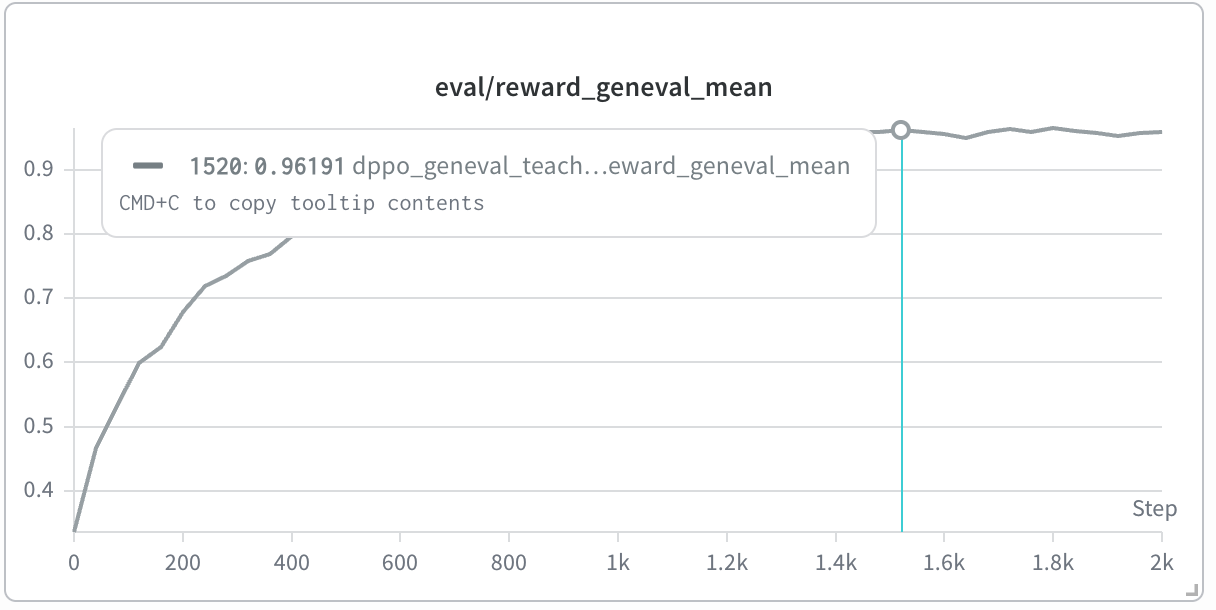
\includegraphics[width=\textwidth]{figures/geneval-teacher-eval.png}
\caption{GenEval --- eval}
\label{fig:teacher_geneval_eval}
\end{subfigure}\hfill
\begin{subfigure}{0.32\textwidth}
\centering
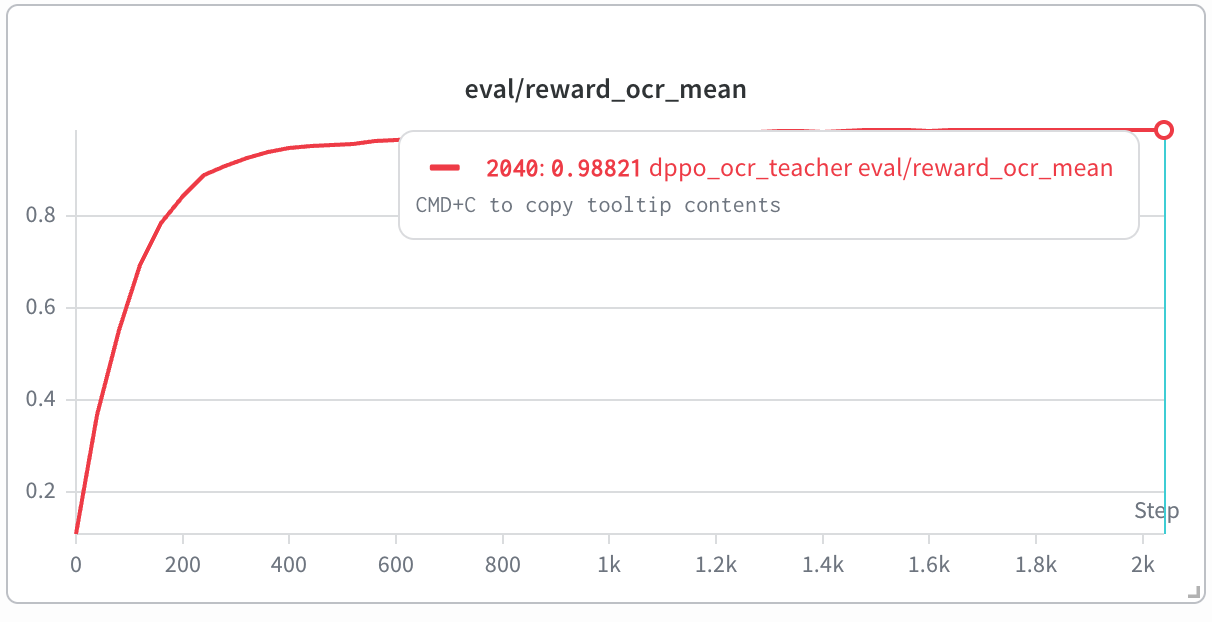
\includegraphics[width=\textwidth]{figures/ocr-teacher-eval.png}
\caption{OCR --- eval}
\label{fig:teacher_ocr_eval}
\end{subfigure}\hfill
\begin{subfigure}{0.32\textwidth}
\centering
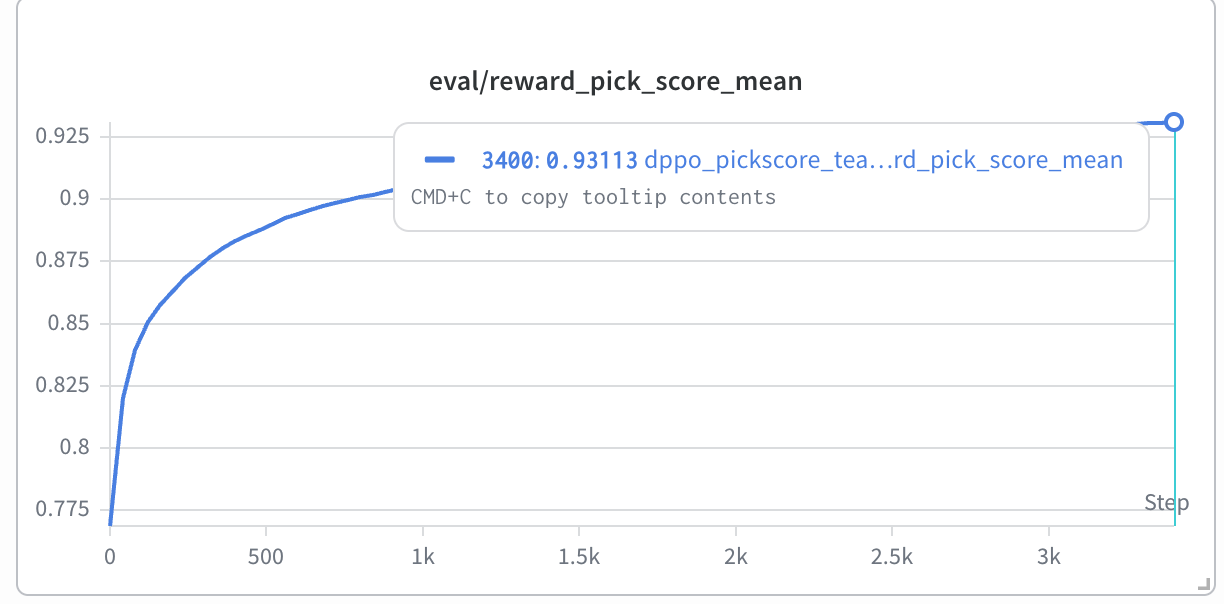
\includegraphics[width=\textwidth]{figures/pickscore-teacher-eval.png}
\caption{PickScore --- eval}
\label{fig:teacher_pick_eval}
\end{subfigure}\\[6pt]
% --- Bottom row: training reward ---
\begin{subfigure}{0.32\textwidth}
\centering
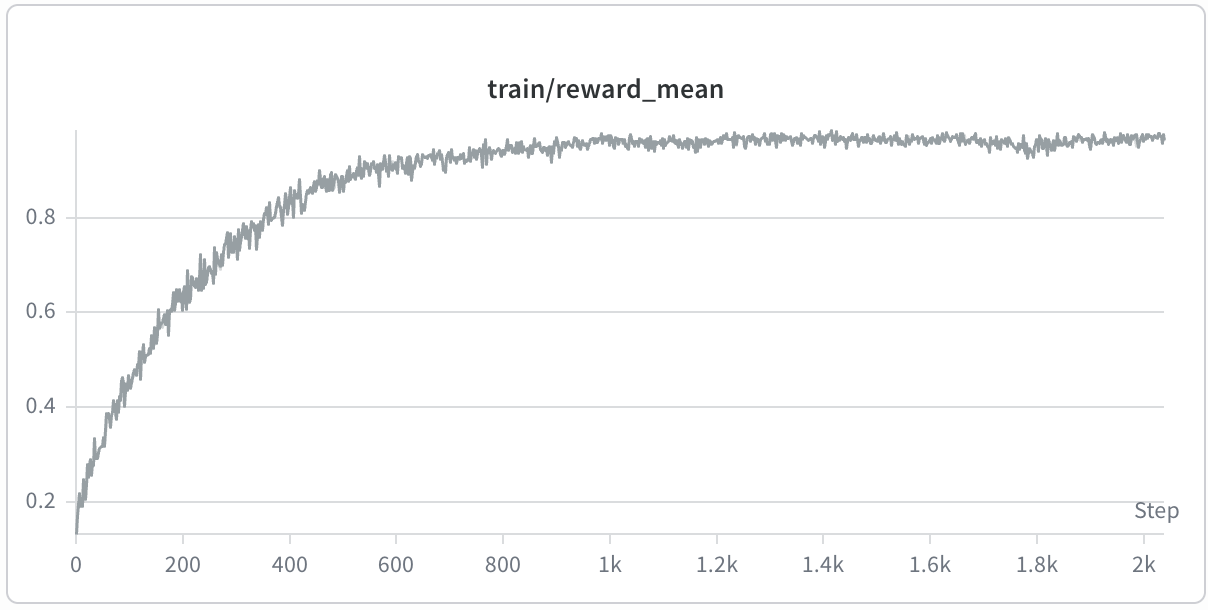
\includegraphics[width=\textwidth]{figures/geneval-teacher-train.png}
\caption{GenEval --- train}
\label{fig:teacher_geneval_train}
\end{subfigure}\hfill
\begin{subfigure}{0.32\textwidth}
\centering
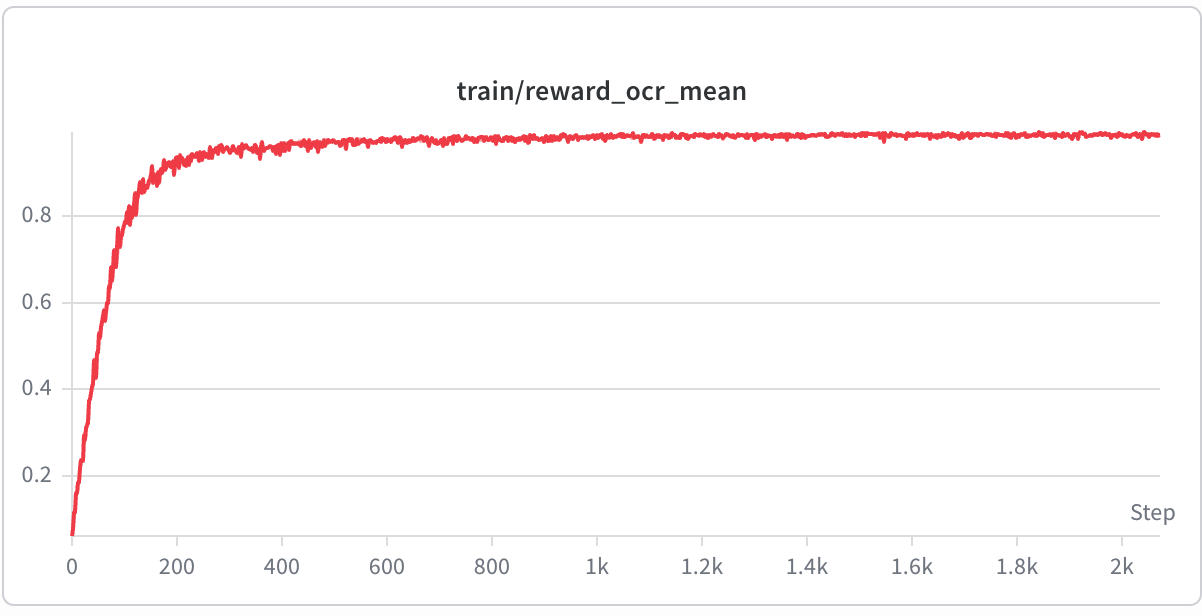
\includegraphics[width=\textwidth]{figures/ocr-teacher-train.png}
\caption{OCR --- train}
\label{fig:teacher_ocr_train}
\end{subfigure}\hfill
\begin{subfigure}{0.32\textwidth}
\centering
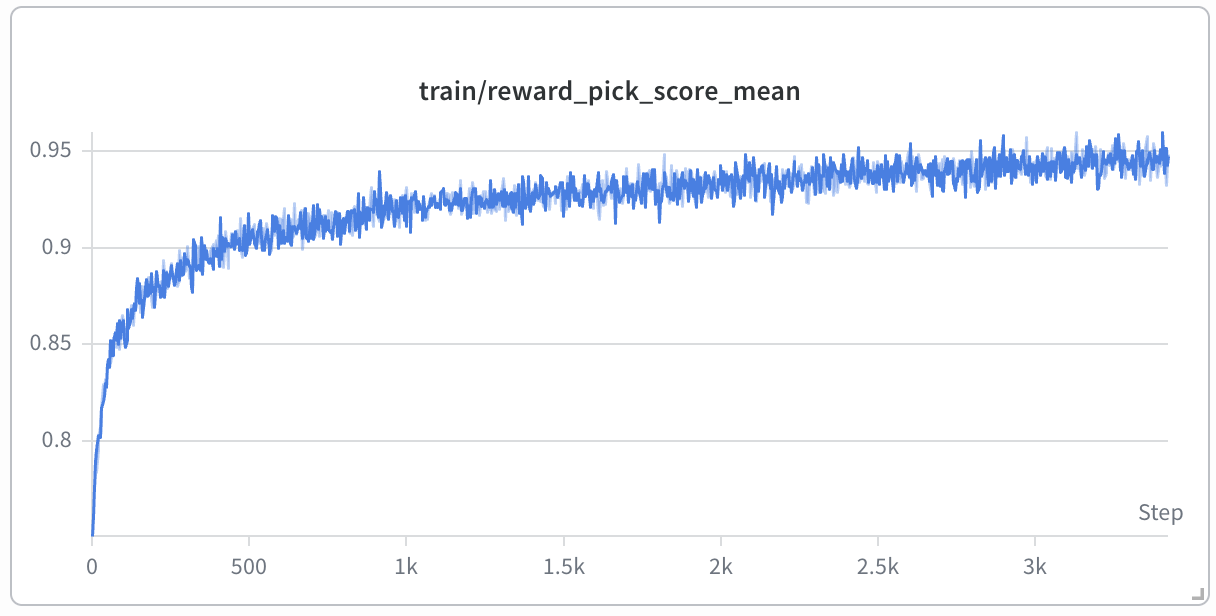
\includegraphics[width=\textwidth]{figures/pickscore-teacher-train.png}
\caption{PickScore --- train}
\label{fig:teacher_pick_train}
\end{subfigure}
\caption{Flow-DPPO teacher 训练曲线（无 CFG）。\textbf{顶行}
（\subref{fig:teacher_geneval_eval}--\subref{fig:teacher_pick_eval}）：
held-out eval reward；\textbf{底行}
（\subref{fig:teacher_geneval_train}--\subref{fig:teacher_pick_train}）：
on-policy 训练 batch reward。MoF 中作为冻结 $v^{(k)}$ 使用的选定
checkpoint 为：GenEval @ step 1200（$R{=}0.958$, ckpt-600），
OCR @ step 440（$R{=}0.953$, ckpt-220），PickScore @ step 3000
（rescaled 后 $R{\approx}0.931$，对应 $\times 26$ 未 rescale 分数 24.128）。
这些选择\emph{保守地早于}图中 tooltip 显示的 peak-reward step；后期
checkpoint 的 reward 仍在攀升但出现质量退化（OCR 尤其会过拟合到
文字检测启发式而牺牲整体图像质量）。三条曲线均已 plateau——单目标
微调收益递减，正是多 teacher mixing 方案变得有吸引力的转折点。}
\label{fig:teacher_training}
\end{figure}

\subsection{MoF 配置}

我们正交消融两个设计轴：
\begin{itemize}[leftmargin=1.5em]
\item \textbf{混合模块}：\texttt{lut}, \texttt{lut\_simple} (LUT-SA),
\texttt{time\_router}, \texttt{adaln\_router}, \texttt{mlp\_router}。
\item \textbf{RL 算法}：DiffusionNFT（默认）, Flow-GRPO。
\end{itemize}

Reward 配置遵循标准的 \emph{per-set composite}：
\begin{equation}
A(x_b, s_b)
= a_{R_{\text{in}}(s_b)}(x_b)
+ \gamma\cdot\frac{1}{|J_b|}\sum_{j\in J_b}a_j(x_b),\qquad
J_b = \{j: j\neq R_{\text{in}}(s_b),\;a_j(x_b)\neq\mathrm{NaN}\},
\label{eq:advantage}
\end{equation}
含三个 reward（GenEval, PickScore, OCR）、三个 source、以及
\texttt{applicable\_sources}：
\texttt{geneval}$\to$\texttt{[geneval]}，
\texttt{pick\_score}$\to$\texttt{[geneval, pickscore, ocr]}（universal），
\texttt{ocr}$\to$\texttt{[ocr]}。默认 $\gamma = 0.2$。

\subsection{评估}

我们同时测量 in-domain 与 OOD 性能：
\begin{itemize}[leftmargin=1.5em]
\item In-domain：每个 $s$ 上的 $f_s^{(s)}(\theta^*)$，与上表的 matched
single teacher eval 分数对比。
\item OOD：$j \neq s$ 时的 $f_j^{(s)}(\theta^*)$，与每个
$f_j^{(s)}(v^{(k)})$ baseline 对比（完整的 $K \times S$ 交叉表）。
\end{itemize}

%% ============================================================
\section{实证发现与消融计划}
\label{sec:exp_findings}
%% ============================================================

\subsection{Pathwise vs.\ PG（验证命题~\ref{prop:pg_zero}）}

在三种模式下跑 Stage-2 蒸馏：\texttt{pathwise\_only},
\texttt{pg\_only}, \texttt{both}。假设：\texttt{pathwise\_only} 与
\texttt{both} 最终 reward 持平；\texttt{pg\_only} 不收敛或训练高方差。
此 ablation 验证 Stage 2 是纯 regression 问题。

\subsection{朴素多 teacher OPD baseline（Step 2）}

两个针对 route-by-source 与 average-velocity baseline 的消融：
\begin{itemize}[leftmargin=1.5em]
\item \textbf{OPD-route}：target $v^{\mathrm{tgt}}(x, t, p) =
v^{(s(p))}(x, t, p)$。假设：in-domain 匹配 teacher（Level-1 平凡），
无 OOD 增益。
\item \textbf{OPD-average}：target $v^{\mathrm{tgt}} = \tfrac{1}{K}
\sum_k v^{(k)}$。假设：由 Jensen 不等式 in-domain 严格退化，OOD 略有
提升。
\end{itemize}
两者作为 MoF 的下界参照点。

\subsection{MoF 主实验：NFT vs.\ Flow-GRPO（Step 3）}

在 LUT 与 adaLN-router 架构上分别用两种 RL 算法跑 MoF。假设：NFT 收敛
更快，最终 reward 接近；Flow-GRPO 需要更多样本但严格 on-policy。每种
设定取 SOTA。

\subsection{$\lambda^*$ 的时序分析}

Stage 1 收敛后，对每个 source $s$ 画 $\lambda_{k, i, s}$ 关于 timestep
$i$ 的曲线。基于已知扩散现象类比的假设：
\begin{itemize}[leftmargin=1.5em]
\item \textbf{早期 timestep（高噪声）}：GenEval-teacher 主导（全局
layout / 物体放置）。
\item \textbf{中期 timestep}：OCR-teacher 贡献（文字笔画形成）。
\item \textbf{晚期 timestep（低噪声）}：PickScore-teacher 主导（美学
精修）。
\end{itemize}

\subsection{NN router 的 PickScore-dominance 失败模式}
\label{ssec:pickscore_dominance}

\textbf{观察}：在初步实验中，神经 router（Time/adaLN/MLP）学出的策略
始终把\emph{所有}样本路由到 \texttt{teacher\_pickscore}，即使在
PickScore-teacher in-domain 表现差的 OCR prompt 上也是如此。LUT 和
LUT-SA \emph{不}出现此失败。

\textbf{机制}（完整推导见
\texttt{mof\_pickscore\_dominance\_analysis.tex}）。因 PickScore 是
\emph{唯一}具有 universal \texttt{applicable\_sources} 的 reward，
PickScore 信号进入\emph{每个}样本的 advantage——一次作为 in-domain
（pickscore 样本），两次通过 OOD bonus（geneval / ocr 样本）。共享参数
$\theta$ 上的总信号覆盖率：
\begin{align}
F_{\text{pick}} &= \tfrac{1}{3}\!\cdot\!1.0 + \tfrac{1}{3}\!\cdot\!\gamma + \tfrac{1}{3}\!\cdot\!\gamma = 0.467,\\
F_{\text{gen}}  &= \tfrac{1}{3}\!\cdot\!1.0 = 0.333,\\
F_{\text{ocr}}  &= \tfrac{1}{3}\!\cdot\!1.0 = 0.333,
\end{align}
所以共享参数 router 上的最优解约偏向 PickScore，比例
$F_{\text{pick}} / F_{\text{ocr}} = 1.4$。LUT 按 source 解耦，每列只
看自己的 $1.0 \!:\! 0.2$ 比例，因此不发展出主导效应。

\textbf{缓解（按推荐优先级）}：
\begin{enumerate}[leftmargin=1.5em]
\item Router 实验中设 $\gamma = 0$（完全放弃 OOD bonus）；
\item 把 PickScore 改为 domain-specific（\texttt{applicable\_sources:[pickscore]}）；
\item 给 router 加 source-conditioning 输入，使其内部能解耦；
\item 按反信号覆盖率重权 per-source advantage。
\end{enumerate}
方案 1 是推荐的第一步。

\subsection{$\gamma$ 消融}

在 adaLN-router 和 LUT 上 grid 扫描
$\gamma \in \{0, 0.05, 0.1, 0.2, 0.5\}$，画 in-domain 与 OOD 分数。
假设：
\begin{itemize}[leftmargin=1.5em]
\item LUT：小 $\gamma$ 改进在 Pareto-friendly range 内单调。
\item Router：$\gamma = 0$ 恢复 OCR；$\gamma > 0$ 触发
PickScore-dominance。
\end{itemize}
此消融把架构因素与 reward 设计因素分离。

\subsection{初始化消融}

对比 \texttt{uniform}, \texttt{random}, \texttt{teacher\_biased}
（in-domain teacher 初始化偏置 $C\!=\!2$）：
\begin{itemize}[leftmargin=1.5em]
\item \texttt{teacher\_biased}：从 Level-1-safe 顶点 $\delta_s^{\const}$
附近出发，应该收敛最快，训练早期 in-domain dip 最小。
\item \texttt{uniform}：从 $1/K$ 出发；学习轨迹必须越过 OPD-Average
中点。
\item \texttt{random}：方差对照。
\end{itemize}

%% ============================================================
\section{讨论}
\label{sec:discussion}
%% ============================================================

\subsection{In-domain 与 OOD 的不对称性}

本框架是根本不对称的：in-domain Level-1 是搜索空间的\emph{结构性}性质
（safe vertex $\delta_s^{\const}$ 始终存在且对复合目标友好），而 OOD
严格超越需要\emph{额外的经验性结构}（时间互补性、梯度对齐、或
非空 Pareto 区域）。从业者不应\emph{先验地}承诺 OOD 改进；应当
\emph{实测}。

\subsection{何时用哪种架构}

简而言之：
\begin{itemize}[leftmargin=1.5em]
\item \textbf{LUT}：适合小 $T, S$（如 $K=3, T=10, S=3$）；消融友好，
因为每个 source/timestep 切片相互独立。
\item \textbf{LUT-SA}：诊断 baseline；用于判断 $S$ 维是否真有用。
\item \textbf{Time Router}：连续 $t$ 灵活性（解耦训练与推理 $T$），
无 prompt conditioning；推荐用于推理 step 消融。
\item \textbf{adaLN/MLP Router}：prompt-conditioned 混合；表达力最强，
但默认 $\gamma$ 下继承 PickScore-dominance 陷阱。
\end{itemize}

决策树：若 reward 配置中存在\emph{universal} reward（覆盖所有 source），
优先用 LUT 或在 router 上设 $\gamma = 0$。若所有 reward 都是
domain-specific 且需要 $T$-灵活性，Time Router 是理想折中。

\subsection{局限}
\begin{itemize}[leftmargin=1.5em]
\item LoRA-shared-base teacher 下，NFT 的梯度量级会变得非常小
（$\sim 10^{-10}$），由 softmax mean-subtraction 导致
（$v^{(j)} - \bar v$ 是小 LoRA residual）。Solutions A--D
（direct-reward, REINFORCE, residual-space, unnormalized）目录见
\texttt{mof\_per\_set\_analysis.tex} \S13--14。
\item Stage 2 蒸馏 gap 是 OOD 增益的主要实践风险；小 margin 可能需要
对 $v^{\MoF^*}$ 做多轮 self-distillation refresh。
\item 所有理论都依赖完美优化（$F^{(s)}$ 全局最大）；实际中小样本量
RL 可能收敛到局部最优，甚至连 Level-1 fallback 都被违反。
\end{itemize}

%% ============================================================
\section{结论}
\label{sec:conclusion}
%% ============================================================

\begin{tcolorbox}[colback=yellow!5,colframe=yellow!60!black,title=核心结论]
\begin{enumerate}[leftmargin=1.5em]
\item Flow matching 框架下的 OPD 蒸馏退化为纯 velocity MSE，因为
policy-gradient 项均值为零（命题~\ref{prop:pg_zero}）。本工作中所有
distillation 都是 regression 问题。
\item 朴素多 teacher OPD 有两类失败模式（route-by-source：无 OOD 增益；
averaging：in-domain 损失）。MoF 用可学习凸组合替代刚性 target——
合法性由命题~\ref{prop:convex_fm} 保证，可在小参数集上用 RL 优化。
\item 理论上 MoF 给出\emph{构造性}的 Level-1 in-domain 保证
（定理~\ref{thm:level1}）、条件性的 Level-2 严格超越
（定理~\ref{thm:level2}）、以及\emph{无}通用 OOD 严格超越保证
（定理~\ref{thm:no_ood}）；不对称性源于缺少复合目标友好的 OOD safe
vertex。
\item 二阶段流水线（RL$\to$distill）解耦 target 优化与部署代价。
NFT 优于 Flow-GRPO（小 mixing 搜索上收敛更快）；$\beta$ 由
定理~\ref{thm:beta_cancel} 不重要。
\item 实践上，当存在 universal reward 时，神经 router 会陷入
PickScore-dominance attractor；LUT 和 LUT-SA 通过 source-decoupling
逃脱该问题。设 $\gamma = 0$ 或限制 \texttt{applicable\_sources} 缓解。
\end{enumerate}
\end{tcolorbox}

\subsection{开放问题}
\begin{enumerate}[leftmargin=1.5em]
\item 设计具有\emph{构造性} OOD fall-back 的 Stage-1 目标
（如 chance-constrained 形式 $\max f_s + \gamma \bar f_{\OOD}$ s.t.\@
$f_j \geq \rho_j^{(s),\const}$）。
\item 比 $q_\theta$ 上 pointwise MSE 更紧的 trajectory-level
distillation loss，降低 Stage-2 erosion。
\item 找到 teacher 集合（LoRA rank、训练数据集）的必要充分条件，
使时间互补性\emph{可证}成立。
\item 把 LUT 的鲁棒性与 router 的 $T$-灵活性结合的 source-conditioned
router with explicit decoupling priors。
\end{enumerate}

%% ============================================================
\appendix
\section{支撑文档索引}
\label{app:supports}
%% ============================================================

本 notes 文档整合了核心叙事；技术推导分散在专题文档中：

\begin{center}
\renewcommand{\arraystretch}{1.4}
\footnotesize
\begin{tabular}{@{}p{5.5cm}p{8cm}@{}}
\toprule
\textbf{主题} & \textbf{文件} \\
\midrule
NFT vs.\ GRPO loss / 梯度对比 &
\texttt{mof\_loss\_gradient\_analysis.tex} \\
NFT 中的 $\beta$ 消去 &
\texttt{nft\_beta\_analysis.tex} \\
Per-set $\lambda$ 架构；梯度消失分析；
solutions A/B/C/D &
\texttt{mof\_per\_set\_analysis.tex} \\
Reward / advantage pipeline 设计 &
\texttt{mof\_reward\_design.tex} \\
连续 router 形式化 &
\texttt{mof\_continuous\_weights.tex} \\
架构数据流（LUT, LUT-SA, Time Router, adaLN, MLP）&
\texttt{mof\_router\_architectures.tex} \\
PickScore-dominance 失败模式分析 &
\texttt{mof\_pickscore\_dominance\_analysis.tex} \\
OOD 严格超越（负面定理；充分条件）&
\texttt{mof\_ood\_guarantee\_analysis.tex} \\
端到端 Stage~1 + Stage~2 流水线；代码索引 &
\texttt{mof\_two\_stage\_pipeline.tex} \\
\bottomrule
\end{tabular}
\end{center}

\section*{参考文献（informal）}
本 notes 把如下作品以纯文本方式行内引用；将 notes 提升为正式 paper 时
需补全完整 BibTeX：
\begin{itemize}[leftmargin=1.5em]
\item \textbf{Flow Matching}（Lipman et al., 2023）。
\item \textbf{Flow-GRPO}, \textbf{DiffusionDPO}, \textbf{DiffusionNFT}
（近期 RL 风格扩散微调工作）。
\item \textbf{OPD}（on-policy distillation 系列工作，包含
multi-teacher route-by-source 变体）。
\item \textbf{Flow-DPPO}（用于训练三个 teacher 的算法）。
\end{itemize}

\end{document}
